\section{Vorwort}
Bei der Recherche zur Bearbeitung der Übungen wurden viele englischsprachige Webseiten zu rate gezogen. Generell kann man sagen, dass englische Fachbegriffe sich im Bereich FPGA und embedded Design etabliert haben, so dass eine Übersetzung eher verwirren als helfen würde. Daher haben wir uns entschieden, die \textbf{englischen} Bezeichner und Beschreibungen beizubehalten.\\
Um Codeabschnitte besser von Beschreibungen besser unterscheiden zu können, wurde eine eigene Schriftart verwendet:
\begin{verbatim}
  Kommandozeilen Eingaben und Codesnippets werden wie HIER dargestellt.
\end{verbatim}

\section{Aufgabe 1} \label{ex1}
In der Laborübung wurde das ZedBoard Zynq-7000 eingesetzt. Es umfasst als \textbf{PL} den Artix-7 FPGA mit 85K Logic Cells (Device Z-7020, Part: XC7Z020) und als \textbf{PS} den Dual-core ARM Cortex-A9 MPCore™ mit 866 MHz.

\begin{minipage}{\textwidth}
    \begin{center}        
        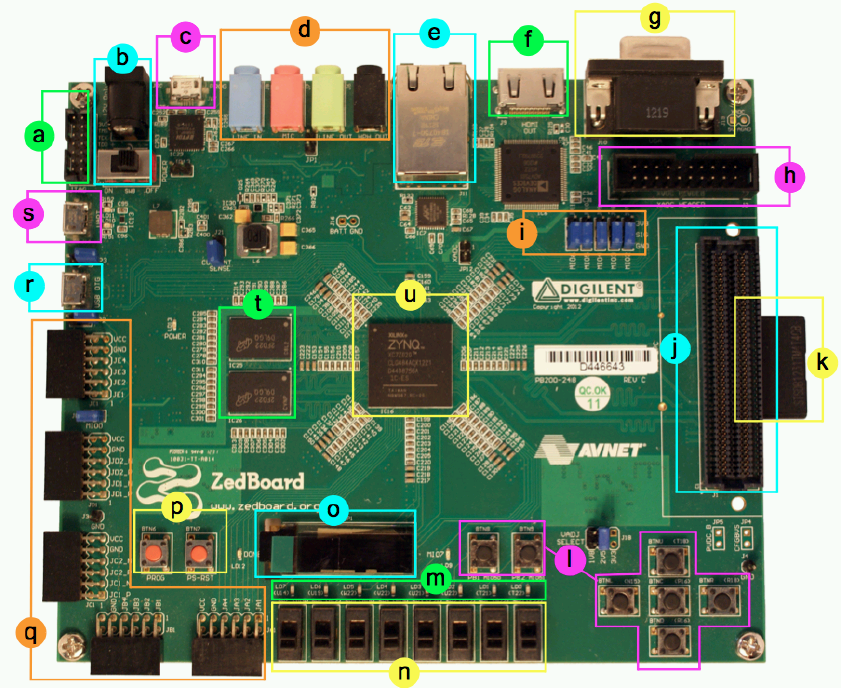
\includegraphics[scale=0.5]{img/a1.png} 
    \end{center}
\end{minipage}
\begin{center}
ZedBoard mit Xilinx Zynq-7000 SoC
\end{center}

Wichtigste Anschlüsse für Laborübung 1
\begin{itemize}
\item b) Power Supply
\item c) USB-JTAG (programming)
\end{itemize}


\subsection{Vorbereitung zur Laborübung}
Memory Mapped I/O und isolated I/O sind zwei Methoden um Input-Output Operationen zwischen CPU und der Peripherie auszuführen.\\

\textbf{Memory Mapped I/O}\\
Es wird der gleiche Adressbus verwendet, um den primären Speicher und den Speicher der Hardwaregeräte anzusteuern. Das bedeutet, die Befehle um bestimmte Bereiche im Speicher anzusprechen, können ebenfalls verwendet werden um die Speicherbereiche der Hardware anzusprechen.\\

\textbf{Isolated I/O}\\
Auf der anderen Seite, verwendet Isolated I/O separate Befehle um den primären und den Gerätespeicher anzusprechen. In einem solchen Fall liegen zwei separate Adressenbereiche vor. Dies können z.B. separate I/O Pins an der CPU oder ein kompletter eigener Bus sein. Da der primäre Speicherbereich von dem Geräteadressbereich getrennt ist, spricht man von Isolated I/O. Isolated IO benötigt spezielle Befehle um zu schreiben und zu lesen.
